\documentclass[]{article}
\usepackage{graphicx}
\usepackage{float}


\graphicspath{{./images/}}
\usepackage[spanish]{babel}
%opening
\title{Resultados de encuesta}
\author{Yael Atletl Bueno Rojas, Kevin Pen\~a Mora, Jos\'e \'Angel }

\begin{document}
	\maketitle
\begin{abstract}
	Se realiz\'o una encuesta dirigida espec\'ificamente a usarios de el motor base para el Framework, para identificar las carencias de \'este y de qu\'e forma se pueden mitigar. 
\end{abstract}
\tableofcontents

\section{Resultados de la encuesta}
\subsection{Estad\'isticas }
\subsubsection{Lugar de procedencia}
\begin{figure}[H]
	
	\centering
	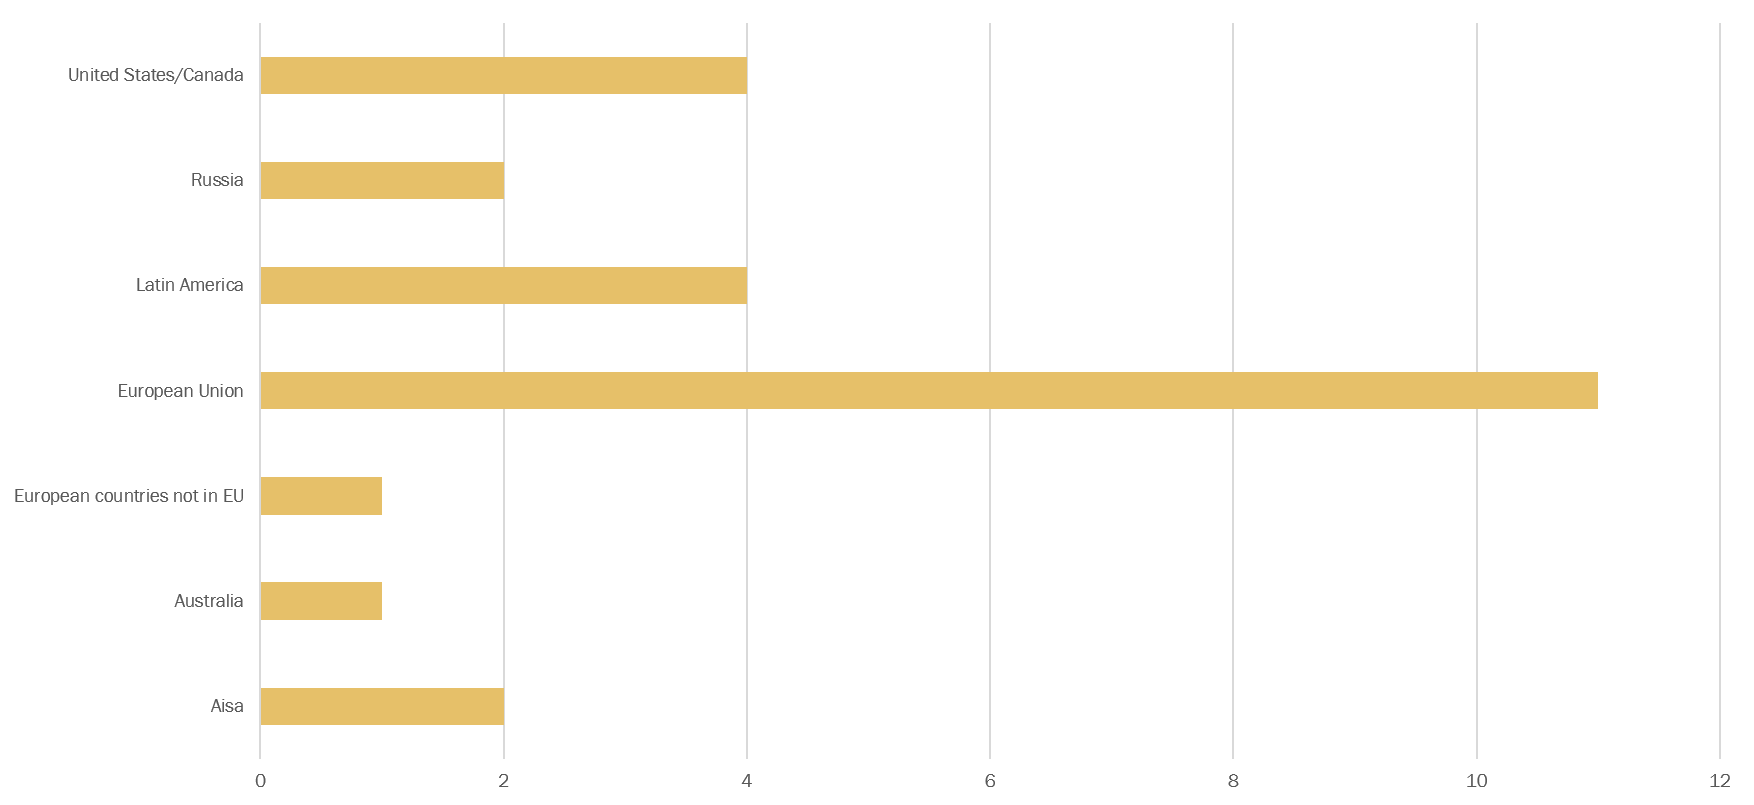
\includegraphics[width=1\textwidth]{Encuesta_lugar}
	\caption{Resultados de la locaci\'on de los usuarios} 
	\label{LUGAR}
	
\end{figure}
Podemos notar que la mayor\'ia de los encuestados provienen de la Uni\'on Europea, seguidos por Estados Unidos, Canad\'a y Latinoam\'erica. V\'ease figura \ref{LUGAR}.

\subsubsection{Edad}
\begin{figure}[H]
	
	\centering
	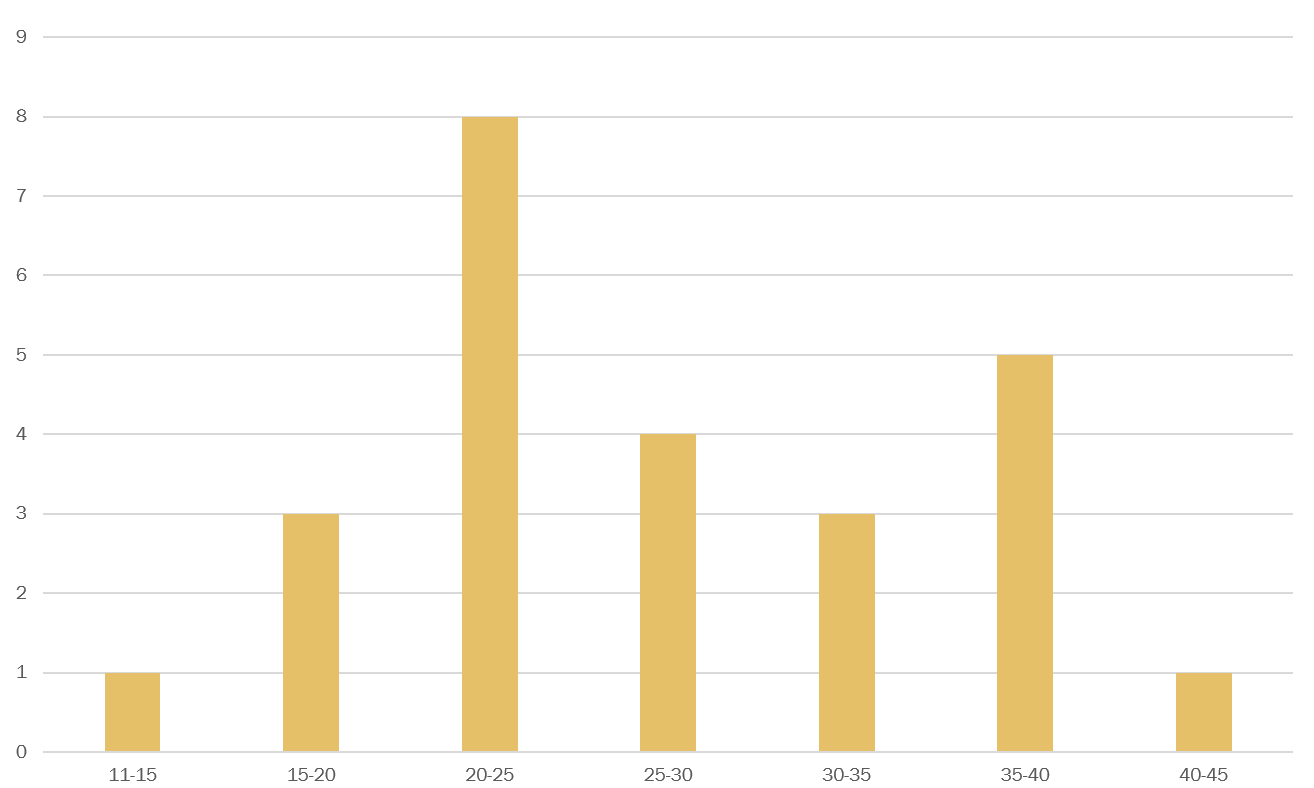
\includegraphics[width=1\textwidth]{Encuesta_edad}
	\caption{Resultados de la edad de los usuarios} 
	\label{EDAD}
	
\end{figure}

En la figura \ref{EDAD} podemos ver que la mayor\'ia de los encuestados tiene entre 15 y 30 a\~nos. 


\subsection{Tiempo de desarrollo}

\subsubsection{Gen\'ericos}
\begin{figure}[H]
	
	\centering
	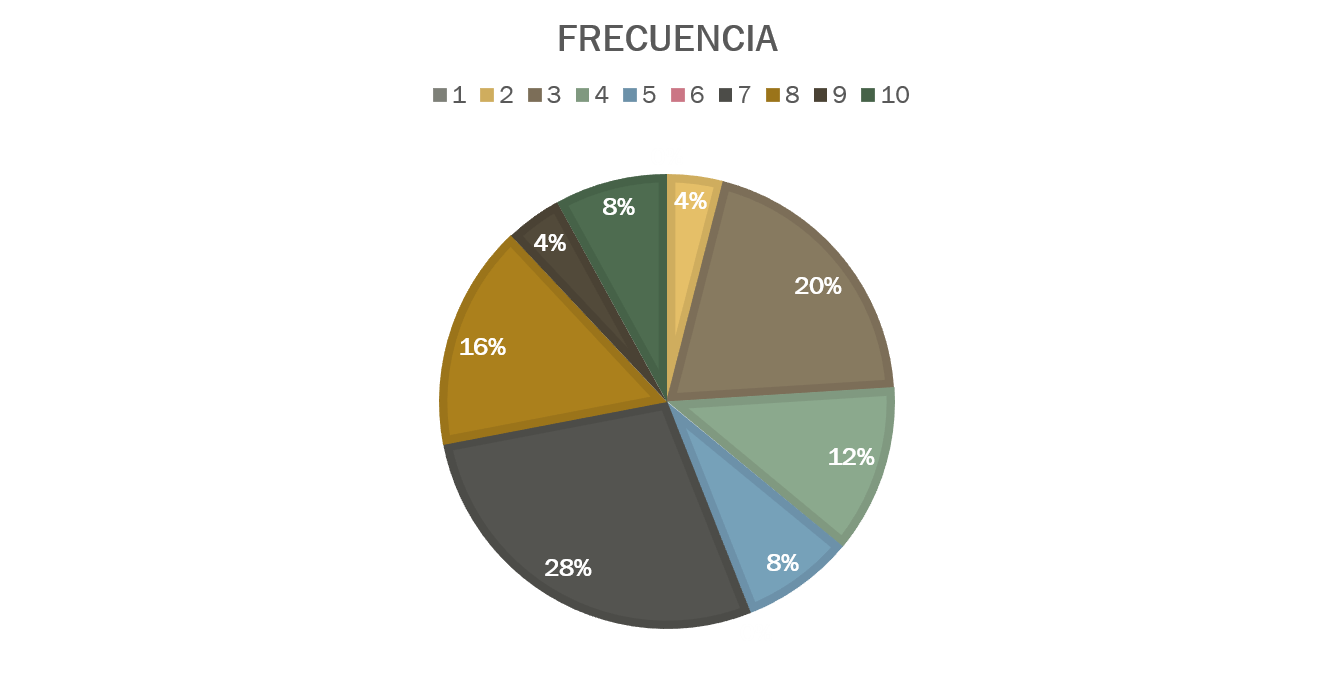
\includegraphics[width=1\textwidth]{Encuesta_tiempo_genericos}
	\caption{En una escala del 1 al 10 con respecto al tiempo total del proyecto.} 
	\label{GENERICO}
	
\end{figure}

De los resultados se ha podido concluir que la mayor\'ia de los programadores pasa de 7/10 a 9/10 del tiempo total del proyecto desarrollando elementos gen\'ericos. Esto es en s\'i conocido como ''reinventar la rueda'' y afecta considerablemente al tiempo de desarrollo negativamente. V\'ease figura \ref{GENERICO}.


\subsubsection{Organizaci\'on de archivos}
\begin{figure}[H]
	
	\centering
	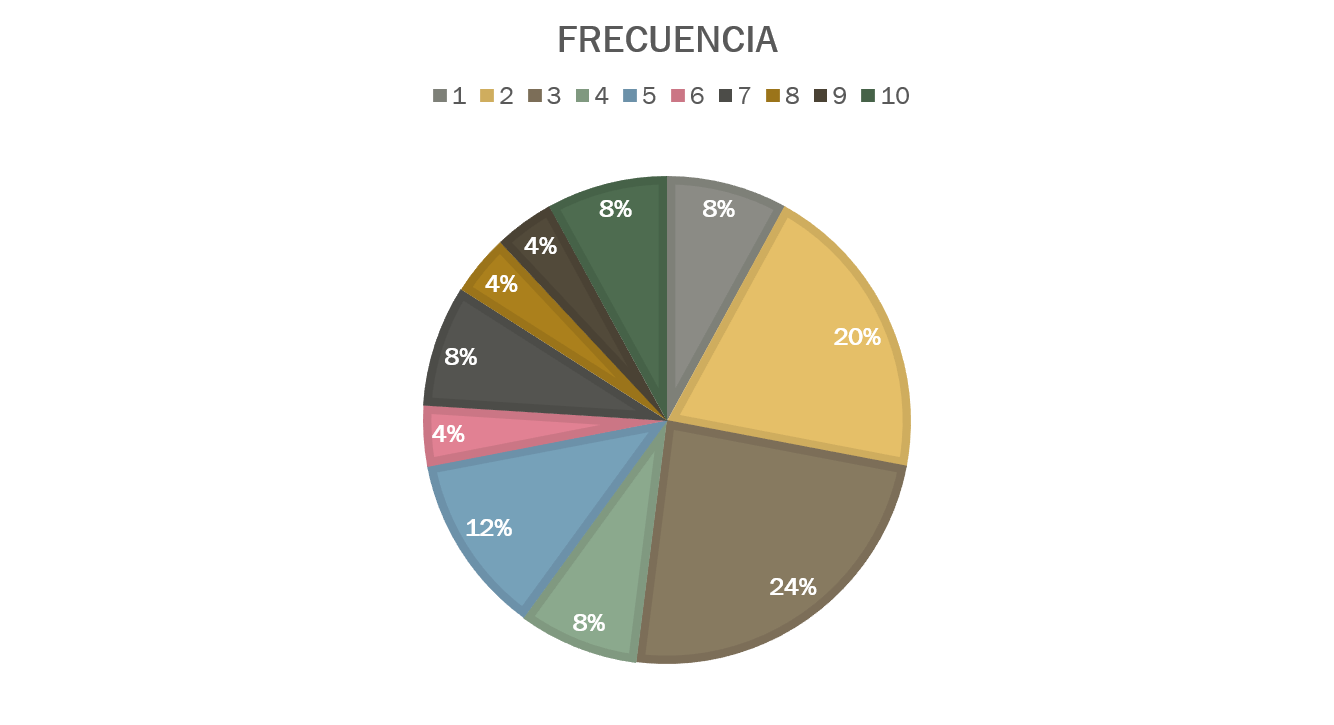
\includegraphics[width=1\textwidth]{Encuesta_tiempo_archivos}
	\caption{En una escala del 1 al 10 con respecto al tiempo total del proyecto.} 
	\label{ARCHIVOS}
	
\end{figure}
En los resultados podemos observar que la gran mayor\'ia de los encuestados no tiene problema alguno con la organizaci\'on de los archivos de su proyecto, lo cual vuelve poco viable crear un administrador para estos. V\'ease figura \ref{ARCHIVOS}.

\subsubsection{Creaci\'on de personajes}
\begin{figure}[H]
	
	\centering
	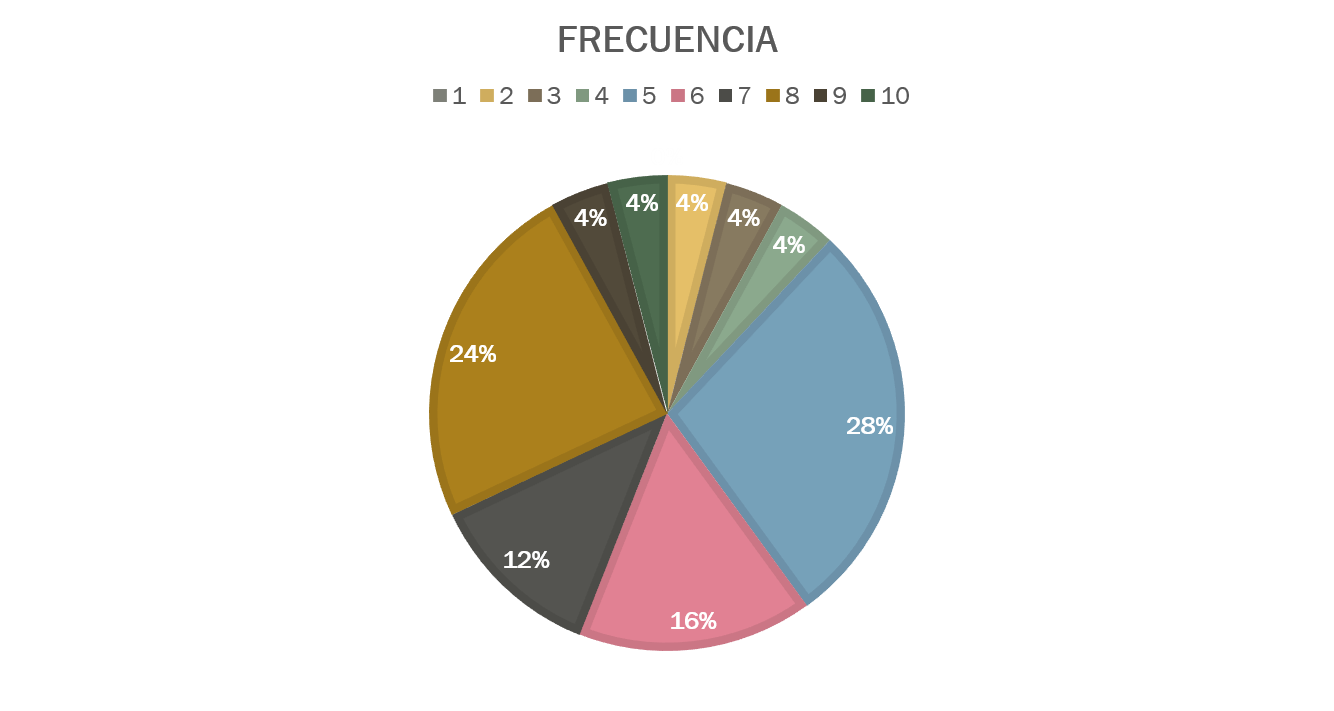
\includegraphics[width=1\textwidth]{Encuesta_tiempo_personajes}
	\caption{En una escala del 1 al 10 con respecto al tiempo total del proyecto.} 
	\label{PERSONAJES}
	
\end{figure}
Se ha concluido que los desarrolladores pasan desde 5/10 hasta 8/10 del tiempo creando sus personajes, proceso que podr\'ia ser acelerado con nuestras herramientas. V\'ease figura \ref{PERSONAJES}.

\subsubsection{Creaci\'on de niveles}
\begin{figure}[H]
	
	\centering
	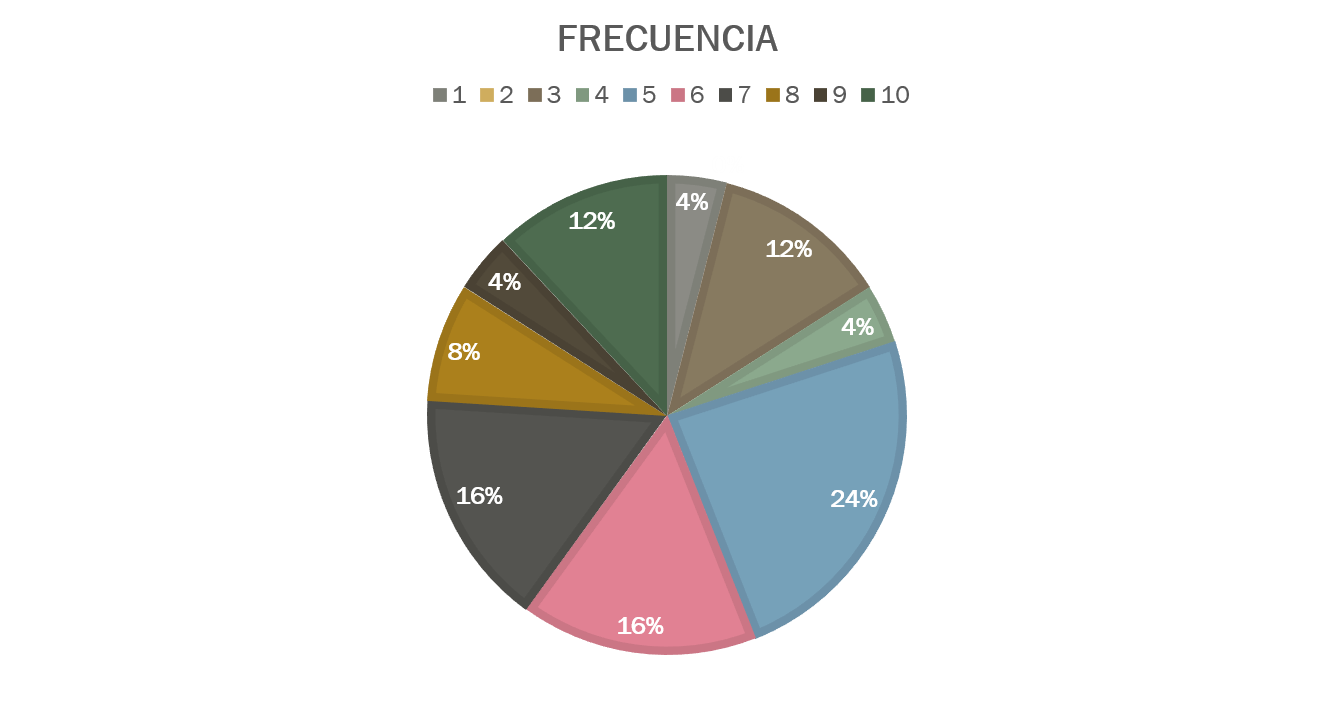
\includegraphics[width=1\textwidth]{Encuesta_tiempo_niveles}
	\caption{En una escala del 1 al 10 con respecto al tiempo total del proyecto.} 
	\label{NIVELES}
	
\end{figure}
Los desarrolladores pasan desde 5/10 hasta 7/10 del tiempo creando sus niveles, proceso que podr\'ia presentar un menor tiempo de desarrollo con ayuda de nuestro editor de niveles procedural. V\'ease figura \ref{NIVELES}.

\subsubsection{Creaci\'on de efectos visuales}
\begin{figure}[H]
	
	\centering
	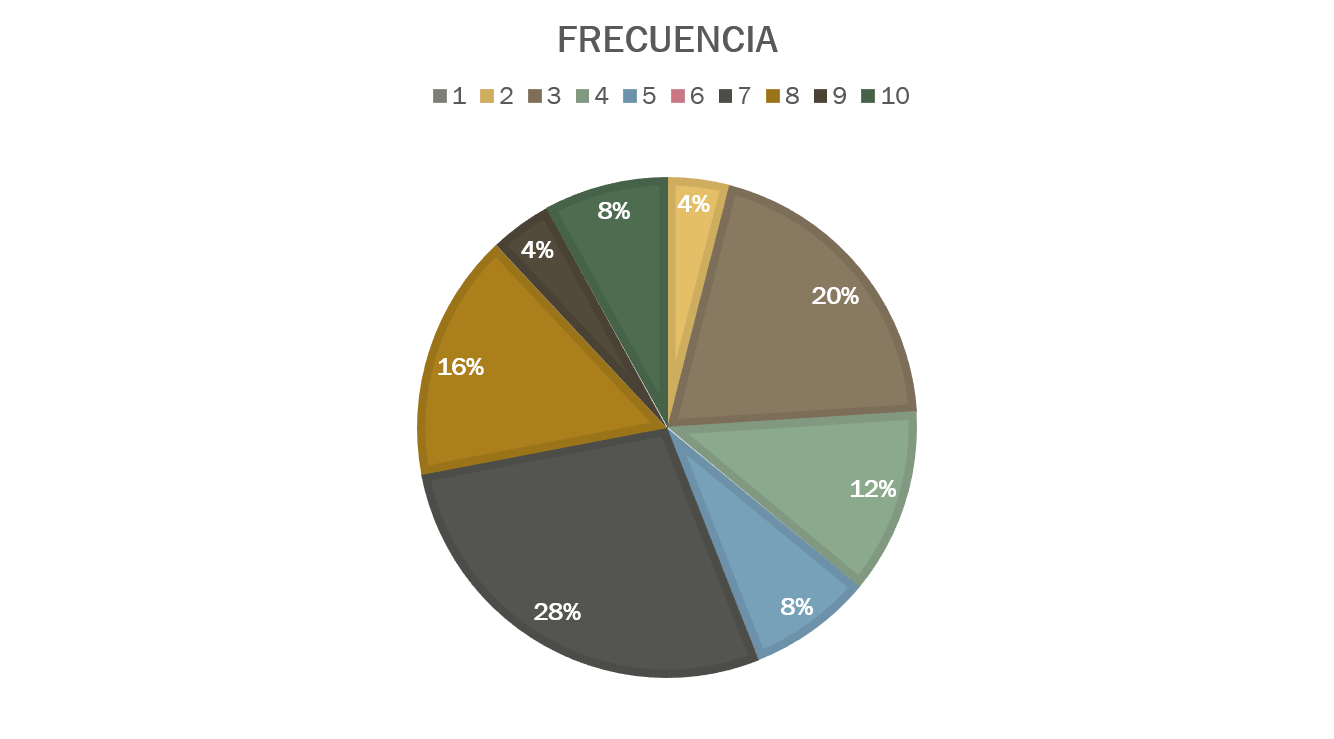
\includegraphics[width=1\textwidth]{Encuesta_tiempo_efectos}
	\caption{En una escala del 1 al 10 con respecto al tiempo total del proyecto.} 
	\label{EFECTOS}
	
\end{figure}
La mayor\'ia de los desarrolladores pasan desde 7/10 a 8/10 del tiempo creando sus efectos especiales. Nuestro editor de part\'iculas y efectos podr\'ia facilitar y reducir el tiempo que toma crear estos mismos. V\'ease figura \ref{EFECTOS}.

\section{Tipo de juego}
\subsubsection{Inclinaci\'on hacia crear un juego Shoot-em-up}
\begin{figure}[H]
	
	\centering
	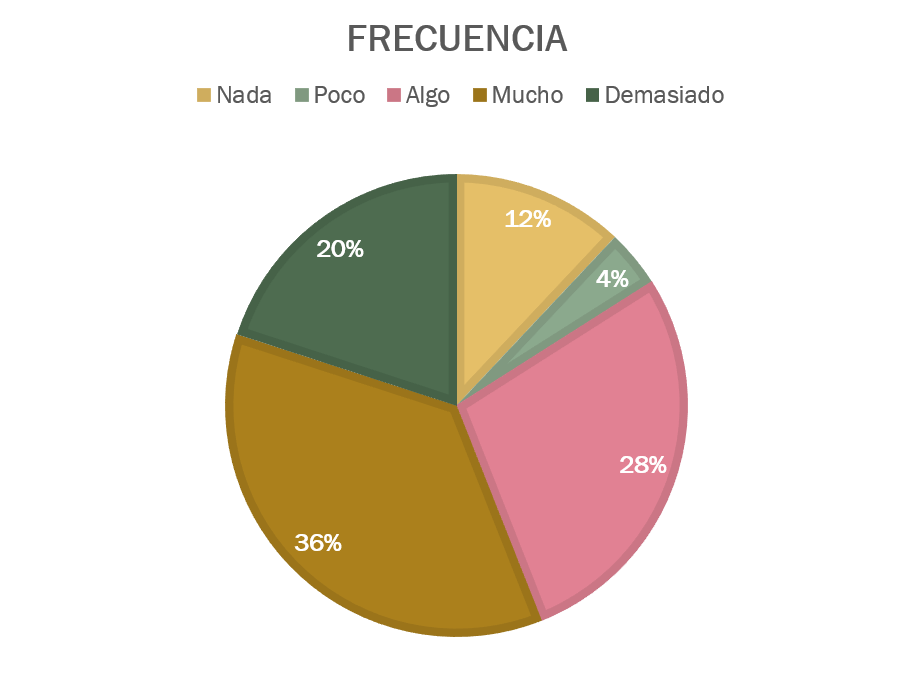
\includegraphics[width=1\textwidth]{Encuesta_tipo_shootemup}
	\caption{En una escala de preferencia, desde nada hasta demasiado} 
	\label{SHOOTEM}
	
\end{figure}
Los desarrolladores tienen una elevada inclinaci\'on a crear Shoot-em-ups lo que se traduce en una inclinaci\'on hacia un ritmo en constante aceleraci\'on y con grandes cantidades de enemigos, lo cual le da importancia a generar una IA optimizada. V\'ease figura \ref{SHOOTEM}.

\subsubsection{Inclinaci\'on hacia crear un juego t\'actico}
\begin{figure}[H]
	
	\centering
	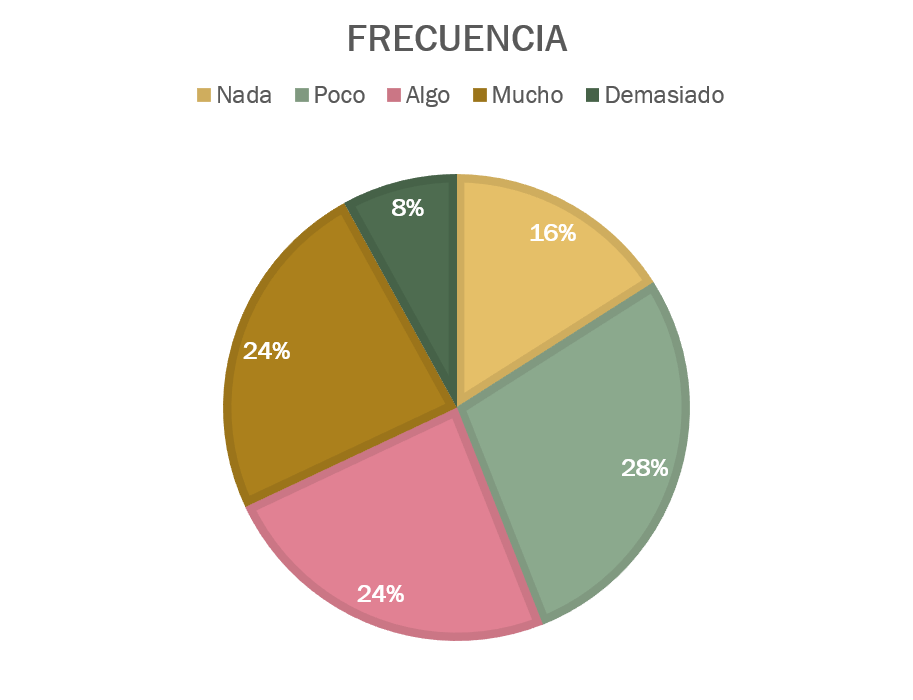
\includegraphics[width=1\textwidth]{Encuesta_tipo_tactico}
	\caption{En una escala de preferencia, desde nada hasta demasiado} 
	\label{TACTICO}
	
\end{figure}
Los desarrolladores tienden a la indiferencia sobre desarrollar un juego t\'actico, siendo s\'olo un 24\% el que demuestra un inter\'es particular hacia el subg\'enero, lo que se traduce en la preferencia de la acci\'on ante la estrategia y la planificaci\'on. V\'ease figura \ref{TACTICO}.
\subsubsection{Inclinaci\'on hacia crear un juego de un s\'olo jugador}
\begin{figure}[H]
	
	\centering
	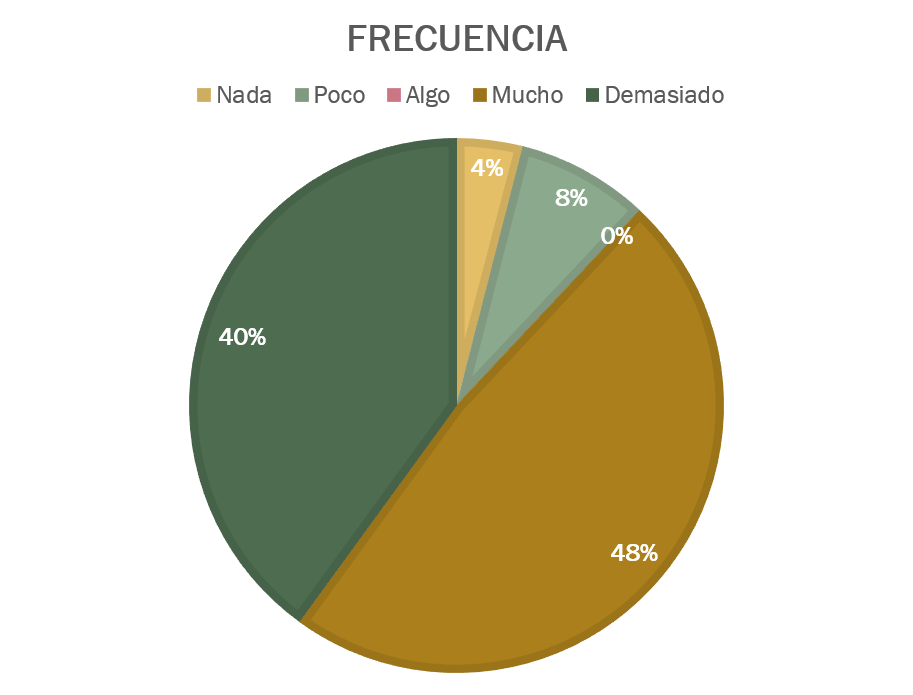
\includegraphics[width=1\textwidth]{Encuesta_tipo_solo}
	\caption{En una escala de preferencia, desde nada hasta demasiado} 
	\label{SOLO}
	
\end{figure}
La preferencia se da hacia las experiencias de un s\'olo jugador, donde un 88\% de los encuestados demostraron inter\'es significativo. V\'ease figura \ref{SOLO}.
\subsubsection{Inclinaci\'on hacia crear un juego multijugador}
\begin{figure}[H]
	
	\centering
	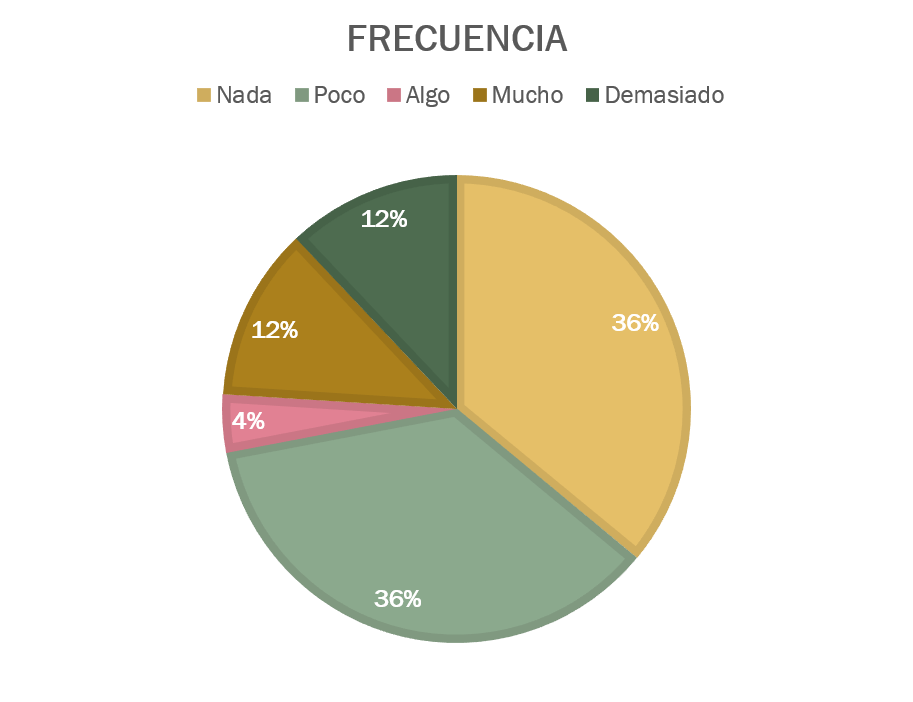
\includegraphics[width=1\textwidth]{Encuesta_tipo_multi}
	\caption{En una escala de preferencia, desde nada hasta demasiado} 
	\label{MULTI}
	
\end{figure}
Los encuestados demostraron gran indiferencia ante este modo de juego, con tan solo un 24\% interesado en \'el. V\'ease figura \ref{MULTI}.

\subsubsection{Inclinaci\'on hacia crear un juego en primera persona}
\begin{figure}[H]
	
	\centering
	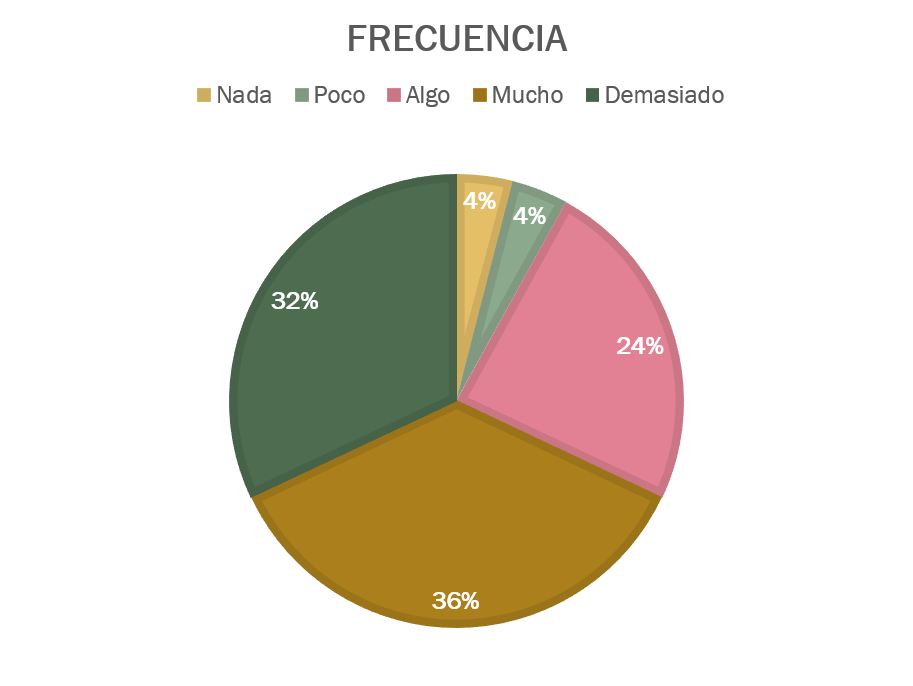
\includegraphics[width=1\textwidth]{Encuesta_tipo_primera}
	\caption{En una escala de preferencia, desde nada hasta demasiado} 
	\label{PRI}
	
\end{figure}
El 64\% demostr\'o inter\'es significativo en esta perspectiva. V\'ease figura \ref{PRI}.
\subsubsection{Inclinaci\'on hacia crear un juego en tercera persona}
\begin{figure}[H]
	
	\centering
	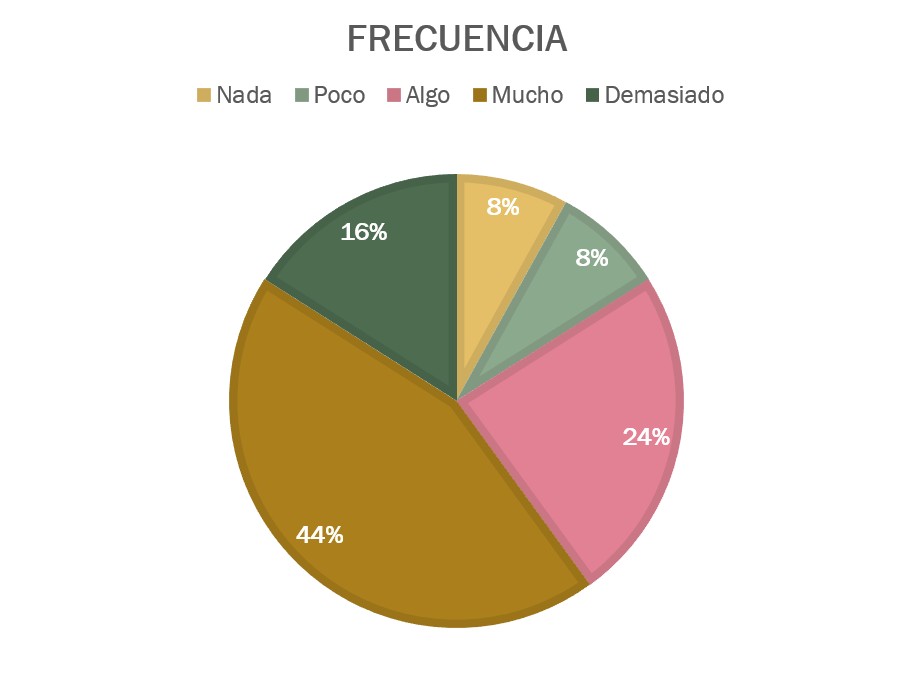
\includegraphics[width=1\textwidth]{Encuesta_tipo_tercera}
	\caption{En una escala de preferencia, desde nada hasta demasiado} 
	\label{TERCERA}
	
\end{figure}
El 60\% demostr\'o inter\'es significativo en esta perspectiva. V\'ease figura \ref{TERCERA}.
\subsection{Facilidad de uso}

\subsubsection{Frecuencia de uso de un editor de personajes}
\begin{figure}[H]
	
	\centering
	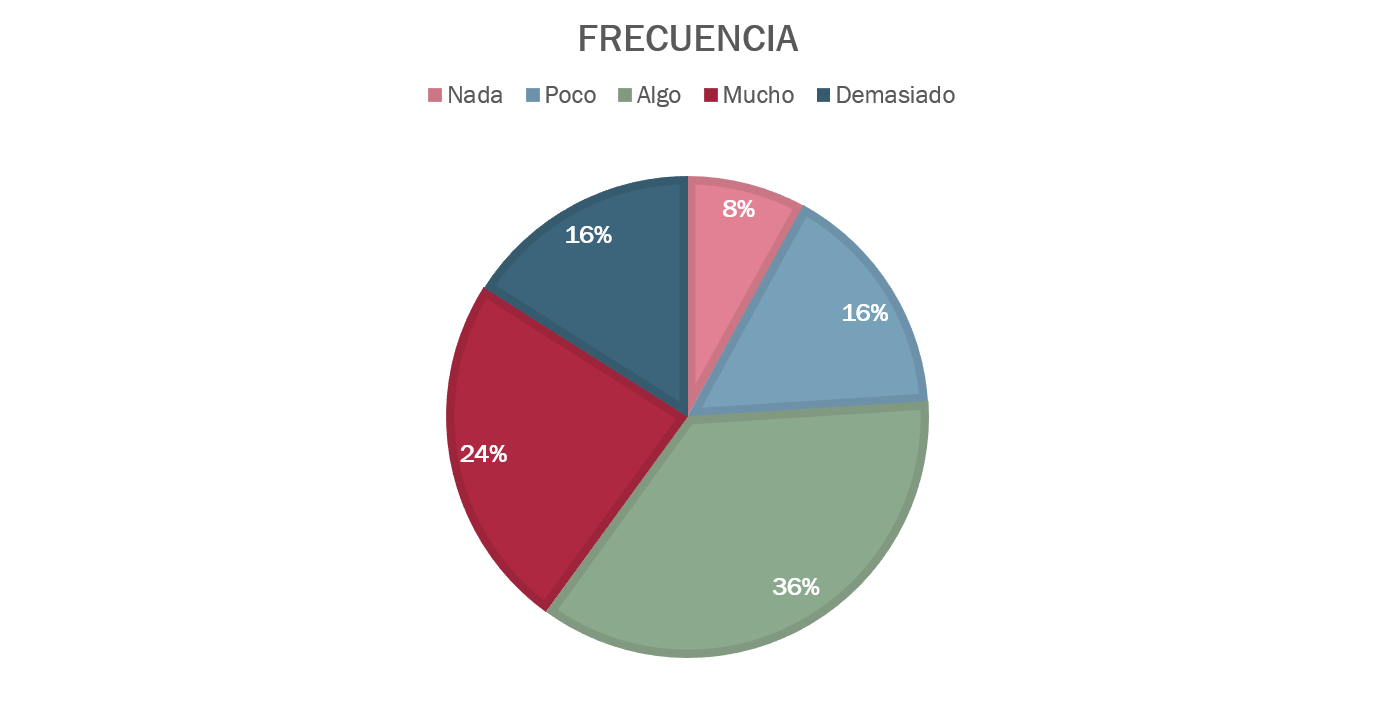
\includegraphics[width=1\textwidth]{Encuesta_facilidad_personajes}
	\caption{En una escala de preferencia, desde nada hasta demasiado} 
	\label{EDITPERS}
	
\end{figure}
El 40\% consider\'o utilizar frecuentemente esta herramienta, mientras que un 36\% consider\'o utilizarla ocasionalmente. V\'ease figura \ref{EDITPERS}.
\subsubsection{Usted es visual}
\begin{figure}[H]
	
	\centering
	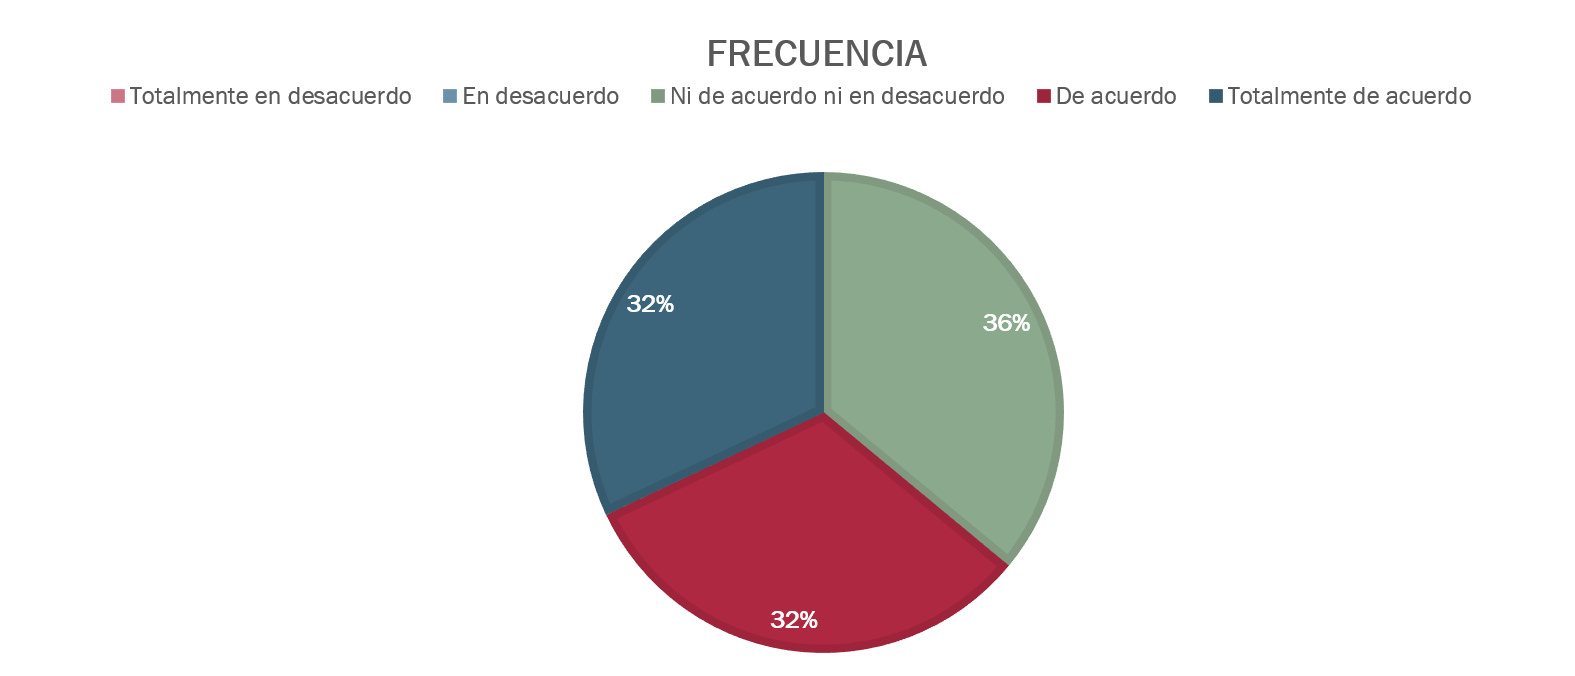
\includegraphics[width=1\textwidth]{Encuesta_facilidad_observacion}
	\caption{En una escala de identificaci\'on con la frase} 
	\label{OBSV}
	
\end{figure}

Los encuestados consideraron ser visuales, se pueden clasificar en mayormente visuales, parcialmente visuales y poco visuales, donde los poco visuales predominan por un 4\%, aunque esto era esperado, considerando que son programadores los que contestaron la encuesta. Sin embargo, si nos enfocamos al porcentaje restante, tendr\'iamos a un 68\% de usuarios que encontrar\'ian convenientes sistemas visuales. V\'ease figura \ref{OBSV}.

\subsubsection{Facilidad de uso de Godot}
\begin{figure}[H]
	
	\centering
	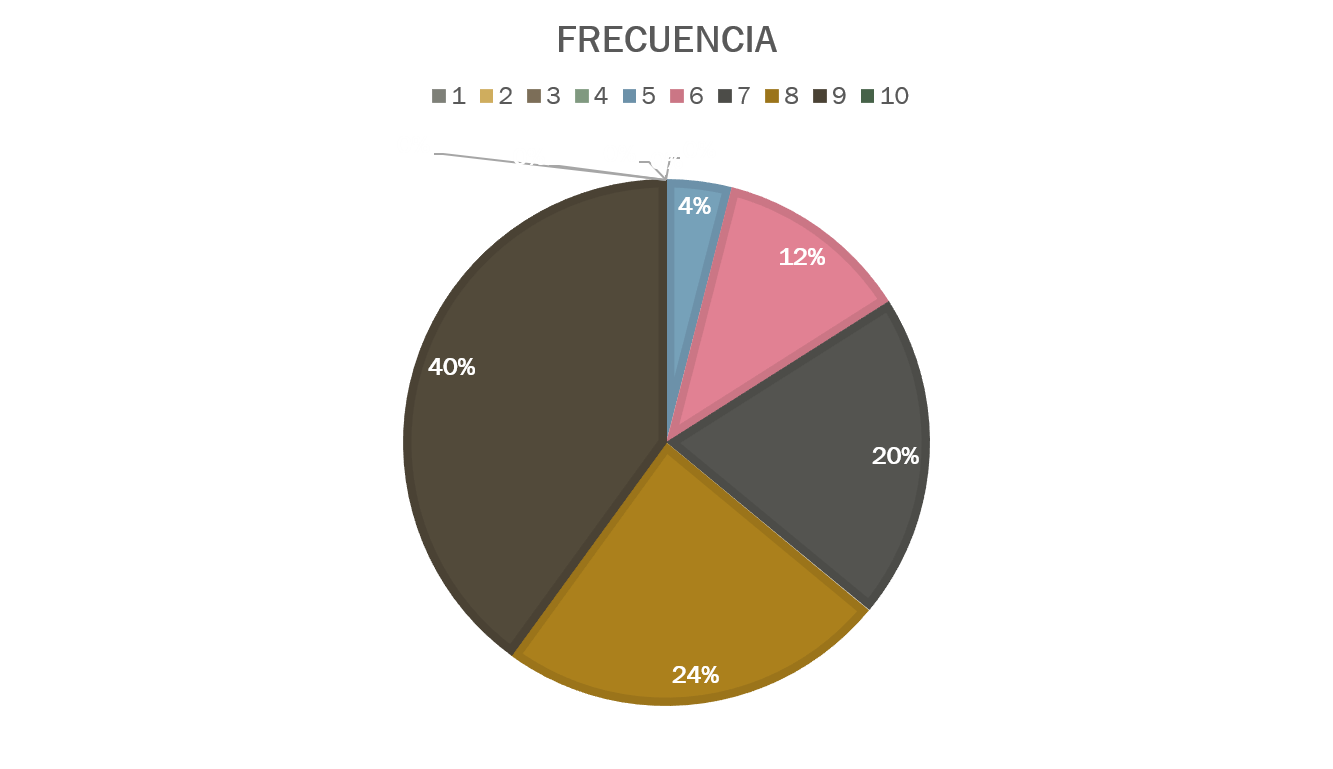
\includegraphics[width=1\textwidth]{Encuesta_facilidad_godot}
	\caption{En una escala de calificaci\'on de satisfacci\'on.}
	\label{GODOT}
	
\end{figure}

Las calificaciones hacia la facilidad de uso de Godot son mayormente positivas, con la calificaci\'on m\'as baja siendo 0 y la m\'as alta 9. La calificaci\'on promedio es 8.  V\'ease figura \ref{GODOT}.
\subsubsection{Facilidad de uso de los pluggins de Godot}
\begin{figure}[H]
	
	\centering
	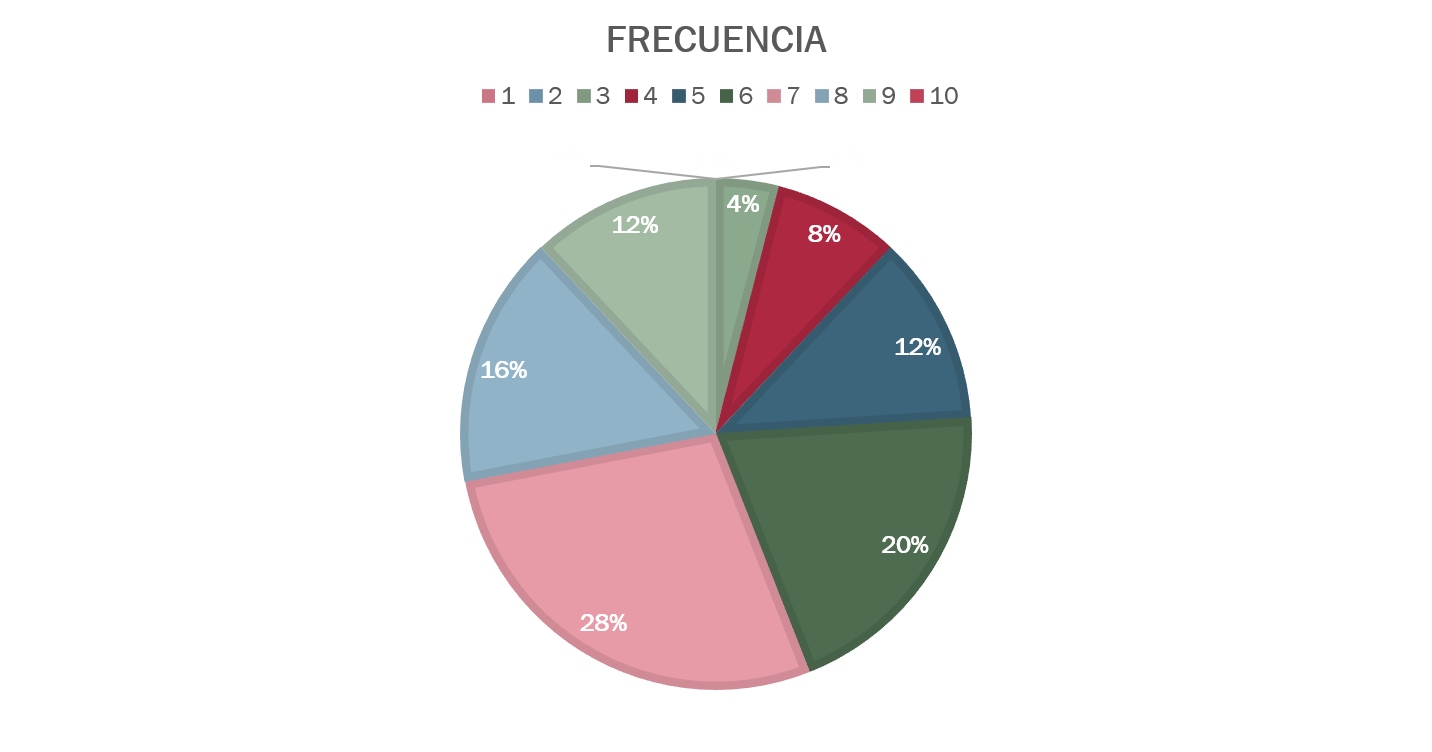
\includegraphics[width=1\textwidth]{Encuesta_facilidad_pluggins}
	\caption{En una escala de calificaci\'on de satisfacci\'on.} 
	\label{PLUG}
	
\end{figure}
La calificaci\'on nos indica que los usuarios no est\'an a gusto con como Godot maneja los plug-ins, teniendo un mayor porcentaje de usuarios que puntuaron en 7. La calificaci\'on promedio es 6.7. V\'ease figura \ref{PLUG}.
\subsubsection{Ejecutable todo en uno}
\begin{figure}[H]
	
	\centering
	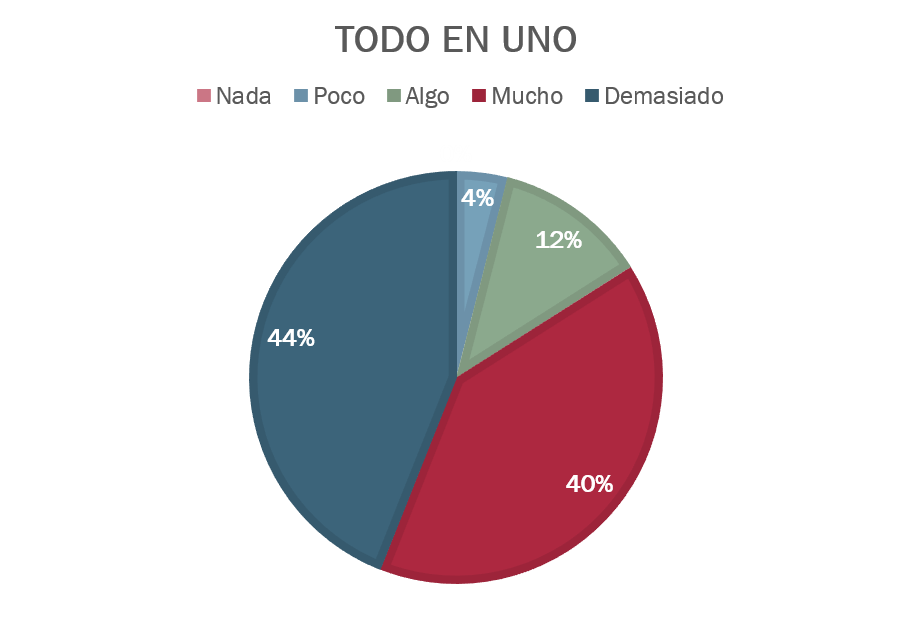
\includegraphics[width=1\textwidth]{Encuesta_facilidad_todoenuno}
	\caption{En una escala de preferencia, desde nada hasta demasiado} 
	\label{ALLINONE}
	
\end{figure}
El 84\% de los encuestados tiene una preferencia hacia los editores compactos, todo en uno. V\'ease figura \ref{ALLINONE}.
\subsubsection{Ejecutables separados por utilidad}
\begin{figure}[H]
	
	\centering
	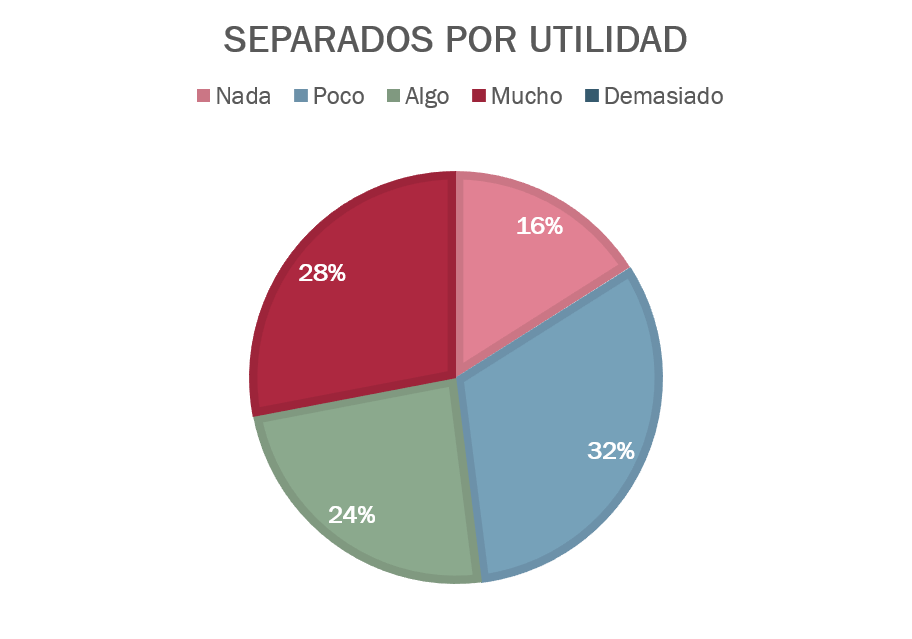
\includegraphics[width=1\textwidth]{Encuesta_facilidad_separados}
	\caption{En una escala de preferencia, desde nada hasta demasiado} 
	\label{SEPARATED}
	
\end{figure}
S\'olo un peque\~o porcentaje de los usuarios tiene preferencia hacia un conjunto de ejecutables con varias herramientas cada uno, la mayor\'ia prefiere otro sistema. V\'ease figura \ref{SEPARATED}.
\subsubsection{Ejecutables con una \'unica utilidad}
\begin{figure}[H]
	
	\centering
	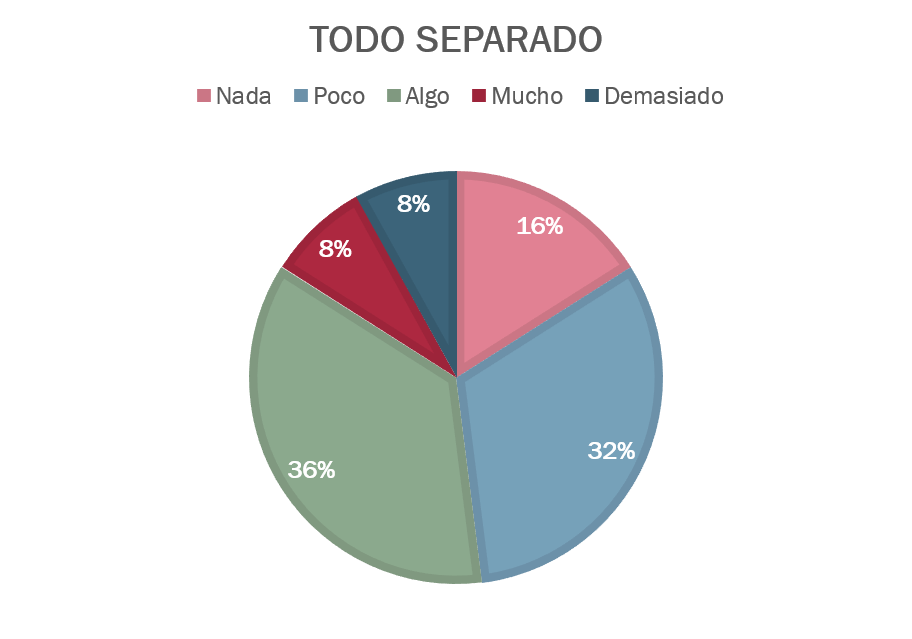
\includegraphics[width=1\textwidth]{Encuesta_facilidad_todoseparado}
	\caption{En una escala de preferencia, desde nada hasta demasiado} 
	\label{DICED}
	
\end{figure}
S\'olo un peque\~o porcentaje de los usuarios tiene preferencia hacia un conjunto de ejecutables con una herramienta cada uno (16\%), la mayor\'ia prefiere otro sistema. V\'ease figura \ref{DICED}.
\section{Conclusiones}
Aqu\'i se tienen los resultados generales y las observaciones obtenidas gracias a la encuesta. 
\subsection{Tiempo de desarrollo}
Los apartados que toman mayor tiempo de desarrollo son los elementos gen\'ericos, los personajes y los efectos, seguidos por los niveles. Se descubri\'o que la organizaci\'on de los archivos no suele ser un problema para los usuarios. 
\subsection{Tipo de juego}
Los resultados apuntan a que el estilo de juego preferido por los desarrolladores es un shooter r\'apido, poco estrat\'egico, en primera o tercera persona y de un s\'olo jugador donde se enfrenten a grandes cantidades de enemigos. 
\subsection{Facilidad de uso}
La preferencia es hacia un sistema visual separado de Godot, contenido en un solo ejecutable, el cual recibir\'ia un uso frecuente de tener un editor de personajes.  
\end{document}
